\documentclass{article}[18pt]
\usepackage{../../../../../format}
\lhead{MCS - Logic and Discrete Structures}
\begin{document}
\begin{center}
\underline{\huge Natural Deduction for Propositional Logic}
\end{center}
\section{Proof Systems for Propositional Logic}
\begin{itemize}
\item What we would like from a proof system
\begin{itemize}
\item \textbf{Completeness} - Using our proof system, we should be able to prove all of the tautologies
\item \textbf{Soundness} - All theorems proved by our proof system should be tautologies
\end{itemize}

\item A \textbf{proof system} defines the proofs (valid mathematical arguments) of the system - it is a collection of \textbf{rules of inference}
\item These rules of inference can be applied to infer new formulae from old
\item Henceforth, we consider propositional logic to consist only of those formulae build using the connectives $\land \lor \lnot \Rightarrow$
\begin{itemize}
\item With other connectives, such as $\Leftrightarrow$, abbreviations
\end{itemize}
\item An \textbf{argument form} in propositional logic is a sequence of formulae\\
$\varphi_1,\varphi_2,...,\varphi_n,\psi$\\
and such an argument form is valid if:
\begin{itemize}
\item Whenever a truth assignment f is s.t. $\varphi_1,\varphi_2,...,\varphi_n$ evaluate to true under f then $\psi$ necessarily evaluates to true under f

\end{itemize}
\item An argument form can also be written in the form $\varphi_1,\varphi_2,...,\varphi_n\vdash\psi$ when it is referred to as a \textbf{sequent}
\item The rule of inference corresponding to the above argument form is:\\
$\varphi_1,\varphi_2,...,\varphi_n\Rightarrow \psi$\\
and if the above argument form is valid then this rule of inference is a \textbf{tautology}
\item The most well known rule of inference for propositional logic is the law of detachment
\end{itemize}
\section{Applying rules of inference}
\begin{itemize}
\item Of course, when applying a rule of inference we can substitute arbitrary formulae for p and q\\
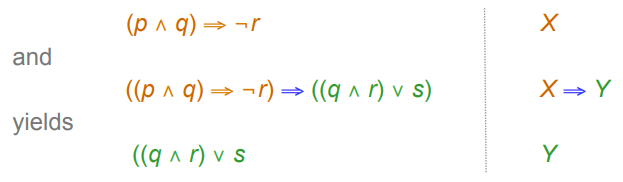
\includegraphics[width=12cm]{Fig1.png}
\item Similarly, given any rule of inference $\varphi_1,\varphi_2,...,\varphi_n\Rightarrow\psi$
\begin{itemize}
\item We can apply this rule by substituting \textbf{any} formula for \textbf{any} propositional variable, so long as the same formula is substituted for the same variable
\item Thus, a valid argument form yields an infinite collection of tautologies
\end{itemize}
\end{itemize}
\section{Other rules of inference}
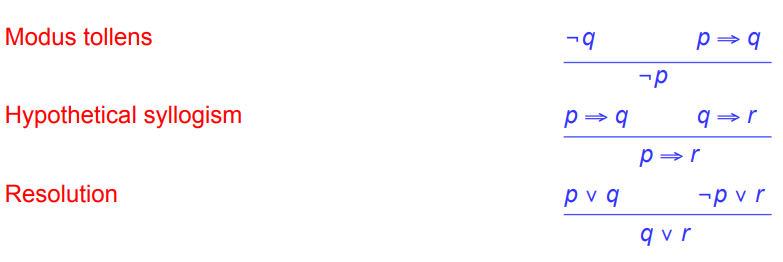
\includegraphics[width=12cm]{Fig2.png}\\
For all these diagrams, if the two statements on the top are true, then the statement on the bottom must be true.
\section{Rules of inference in action}

\section{An alternative approach}
\begin{itemize}
\item We could write down all possible truth assignments on A,W,I,P,S and D, and:
\begin{itemize}
\item Retain only those for which\\
$A\land W\Rightarrow I,A\lor P,W\lor S, \lnot I$ and $D\Rightarrow \lnot (P\lor S)$\\
are true
\item Then check to see that for all of these retained truth assignments we have that $\lnot D$ is true
\end{itemize}
\item However, this would mean that $2^6=64$ different truth assignments need to be checked
\item Consequently, the proof-theoretic approach can be significantly more efficient than the truth table approach, especially when there is a large number of propositional variables
\item Of course knowing which rules of inference to apply which formulae so that we get a speedy proof is another difficulty that needs to be overcome
\end{itemize}
\section{Natural Deduction}
\begin{itemize}
\item The proof system \textbf{natural deduction} consists of a collection of valid rules of inference and is used to obtain proofs of sequence of the form:\\
$\varphi_1,\varphi_2,...,\varphi_n\vdash \psi$
\item We assume that we are given $\varphi_1,\varphi_2,...,\varphi_n$ as \textbf{premises}. We hope to apply our rules of inference from the proof system to obtain $\psi$
\item Rules for conjunction:\\
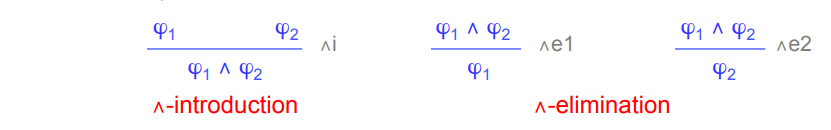
\includegraphics[width=12cm]{Conjunction.png}
\item Rules for double negation:\\
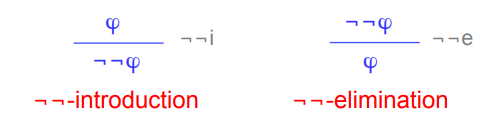
\includegraphics[width=8cm]{Negation.png}
\item Note
\begin{itemize}
\item In general $\varphi_1$ and $\varphi_2$ are formulae and not necessarily propositional variables
\item All of our rules are valid
\end{itemize}
\end{itemize}
\section{A simple proof}
\begin{itemize}
\item Here is the proof of the sequent $p,\lnot\lnot (q\land r)\vdash \lnot \lnot p \land r$ using the rules we have introduced so far\\
\begin{tabular}{l l l }
1&p&premise\\
2&$\lnot\lnot (q\land r)$&premise\\
3&$\lnot\lnot p$&$\lnot \lnot i1$\\
4&$q\land r$&$\lnot\lnot e 2$\\
5&r&$\land e2 4$\\
6&$\lnot\lnot p\land r$&$\land i 3 5$ 

\end{tabular}
\item Note that the validity of the rules means that
\begin{itemize}
\item If p and $\lnot \lnot(q\land r)$ are true under some truth assignment then $\lnot \lnot p\land r$ is necessarily true under this truth assignment
\end{itemize}
\item We often say that a sequent is \textbf{valid} if it can be proved
\end{itemize}
\section{More rules}
\begin{itemize}
\item Rule for eliminating implication\\
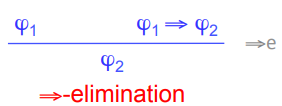
\includegraphics[width=5cm]{Fig3.png}
\item Rule for introducing implication\\
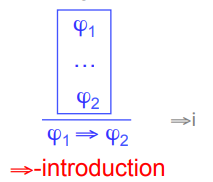
\includegraphics[width=4cm]{Fig4.png}
\item The box doesn't imply $\varphi_1$ is true, just that the stuff below the line is true if the stuff above the line is true
\item In order to apply the rules $\Rightarrow i$
\begin{itemize}
\item To start with the intended premise $\varphi_1$, as the first line of the box
\item Continue until we prove $\varphi_2$
\item Close the box and write our implication $\varphi_1\Rightarrow\varphi_2$
\end{itemize}
\item Thereafter we are not allowed to use any formula in the box. Once a box has closed then the formula within it are no longer available to us
\end{itemize}
\section{Proof using boxes}
\begin{itemize}
\item Here is a proof of the sequent $p\Rightarrow q, q\Rightarrow r \vdash p \Rightarrow r$\\
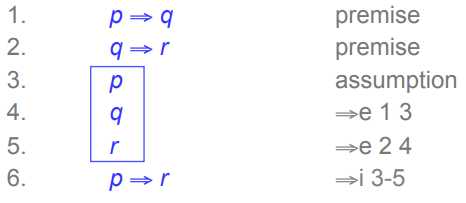
\includegraphics[width=7cm]{Fig5.png}
\item Note that it is possible
\begin{itemize}
\item For a proof to involve more than one box
\item For boxes to be nested within each other
\end{itemize}
\item Note that boxes cannot overlap
\begin{itemize}
\item We cannot \textbf{open} a box and then \textbf{open} another box, then \textbf{close} the first box before \textbf{closing} the second box
\end{itemize}
\end{itemize}
\section{More than one box}
\begin{itemize}
\item Here is a proof of the sequent $(p\land q)\Rightarrow r \vdash p\Rightarrow(q\Rightarrow r)$\\
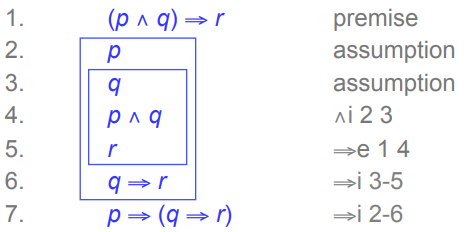
\includegraphics[width=7cm]{Fig6.png}
\item Note that the structure of the formula we wish to prove helps to determine the structure/tactics of our proof
\end{itemize}


\end{document}